\subsection{Ismertesse a diszkrét idejű konvolúció szerepét, összefüggését!}

\noindent \textbf{Konvolúció:}
\begin{itemize}
    \item bevezetünk ún. „egységnyi” jeleket – vizsgálójeleket
    \item ebből tudunk következtetni a rendszer tetszőleges bemenetre adott válaszára
    \item összetett bemenő jelek válaszának meghatározása komponensekre bontással:
    \begin{itemize}
        \item a bemenőjelet vizsgálójelekből álló komponensekre bontjuk
        \item meghatározzuk az elemi komponensek elemi hatását
        \item az időinvariancia és a szuperpozíció elvének kihasználásával az elemi hatásokat összegezzük
    \end{itemize}
    \item diszkrét idejű egységimpulzus:
    $$ \delta[k] = \begin{cases} 0 \text{ ha } k \neq 0 \\ 1 \text{ ha } k = 0 \end{cases} \quad k \in \mathbb{Z} $$
    \begin{itemize}
        \item eltolás esetén:
        $$ \delta[k-K] = \begin{cases} 0 \text{ ha } k \neq K \\ 1 \text{ ha } k = K \end{cases} \quad k, K \in \mathbb{Z} $$
        \item szorzás esetén
        $$ Y_0 \delta[k] = \begin{cases} 0 \text{ ha } k \neq 0 \\ Y_0 \text{ ha } k = 0 \end{cases} \quad k \in \mathbb{Z}, \quad Y_0 \in \mathbb{R} $$
    \end{itemize}
    \begin{figure}[H]
        \centering
        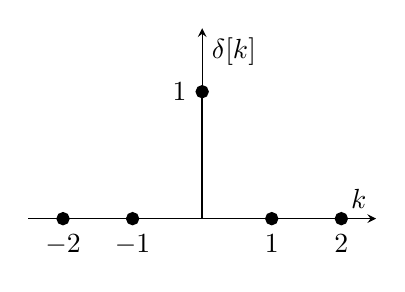
\begin{tikzpicture}
            \begin{axis}[
                width=6cm, height=4cm,
                axis lines=middle,
                xlabel=$k$, ylabel={$\delta[k]$},
                xmin=-2.5, xmax=2.5,
                ymin=0, ymax=1.5,
                xtick={-2,-1,0,1,2},
                ytick={1},
            ]
                \addplot[black, thick, ycomb, mark=*] coordinates {(-2,0) (-1,0) (0,1) (1,0) (2,0)};
            \end{axis}
        \end{tikzpicture}
    \end{figure}

    \item diszkrét idejű egységugrás:
    $$ \varepsilon[k] = \begin{cases} 0 \text{ ha } k < 0 \\ 1 \text{ ha } k \geq 0 \end{cases} \quad k \in \mathbb{Z} $$
    \begin{itemize}
        \item eltolás esetén:
        $$ \varepsilon[k-K] = \begin{cases} 0 \text{ ha } k < K \\ 1 \text{ ha } k \geq K \end{cases} $$
        \item szorzás esetén:
        $$ Y_0 \varepsilon[k] = \begin{cases} 0 \text{ ha } k < 0 \\ Y_0 \text{ ha } k \geq 0 \end{cases} \quad k, K \in \mathbb{Z} \quad Y_0 \in \mathbb{R} $$
    \end{itemize}
    \begin{figure}[H]
        \centering
        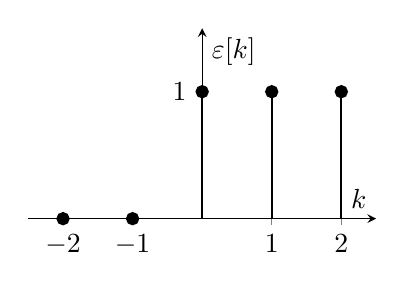
\begin{tikzpicture}
            \begin{axis}[
                width=6cm, height=4cm,
                axis lines=middle,
                xlabel=$k$, ylabel={$\varepsilon[k]$},
                xmin=-2.5, xmax=2.5,
                ymin=0, ymax=1.5,
                xtick={-2,-1,0,1,2},
                ytick={1},
            ]
                \addplot[black, thick, ycomb, mark=*] coordinates {(-2,0) (-1,0) (0,1) (1,1) (2,1)};
            \end{axis}
        \end{tikzpicture}
    \end{figure}

    \item amikor egy diszkrét idejű rendszernek a bemenő jele egy diszkrét idejű egységimpulzus, akkor a kimenő jelet súlyfüggvénynek (vagy impulzusválasznak) nevezzük
    \begin{itemize}
        \item jele: $w[k]$
    \end{itemize}
    \item vizsgálójelek alapösszefüggései:
    $$ \sum_{i=-\infty}^{\infty} \delta[i] = 1 $$
    \item belátható, hogy egy diszkrét idejű függvény konvolúciója az egységimpulzussal egy adott K érték mellett a függvény K helyen felvett értékét adja vissza
    $$ y[K] = \sum_{i=-\infty}^{\infty} y[i] \delta[K-i] = \sum_{i=-\infty}^{\infty} y[K-i] \delta[i] \quad K \in \mathbb{Z} $$
    \item az egységugrás értéke a k helyen kiszámolható az egységimpulzus függvényből
    $$ \varepsilon[k] = \sum_{i=-\infty}^{k} \delta[i] \quad k \in \mathbb{Z} $$
    \item az egységugrás két szomszédos helyen felvett értéknek különbsége megegyezik az egységimpulzus függvény megfelelő helyen felvett értékével
    $$ \delta[k] = \varepsilon[k] - \varepsilon[k-1] \quad k \in \mathbb{Z} $$
    \item egy diszkrét idejű rendszer kimenete k-adik időpillanatban a súlyfüggvénnyel és a bemenettel felírva:
    $$ y[k] = \sum_{i=0}^{k} w[k-i]u[i] \quad k \geq 0 $$
    \item mivel $w[k-i]u[i]$ az i-edik időpillanat bemenetének a kimenetre való hatása
    $$ u[k=K] = u[k=K]\delta[(k-K)=0] $$
    $$ y[k] = \sum_{i=0}^{k} w[k-i]u[i] \quad k > 0 $$
    
    \begin{figure}[H]
        \centering
        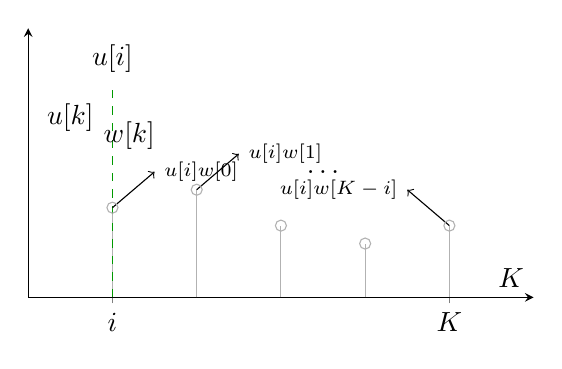
\begin{tikzpicture}
            \begin{axis}[
                width=8cm, height=5cm,
                axis lines=middle,
                xlabel=$K$, ylabel=\empty,
                xmin=0, xmax=6,
                ymin=0, ymax=1.5,
                xtick={1, 5},
                xticklabels={$i$, $K$},
                ytick=\empty
            ]
                % u[k] impulses (schematic representation)
                \addplot[black!30, thin, ycomb, mark=o] coordinates {(1,0.5) (2,0.6) (3,0.4) (4,0.3) (5,0.4)};
                
                % Highlighted impulse at i
                \draw[dashed, green!60!black] (axis cs:1,0) -- (axis cs:1,1.2) node[above, black] {$u[i]$};
                
                % Labels
                \node at (axis cs:0.5, 1) {$u[k]$};
                \node at (axis cs:1.2, 0.9) {$w[k]$};
                
                % Arrows indicating contribution
                \draw[->] (axis cs:1,0.5) -- (axis cs:1.5,0.7) node[right, font=\scriptsize] {$u[i]w[0]$};
                \draw[->] (axis cs:2,0.6) -- (axis cs:2.5,0.8) node[right, font=\scriptsize] {$u[i]w[1]$};
                \node at (axis cs:3.5, 0.7) {$\dots$};
                \draw[->] (axis cs:5,0.4) -- (axis cs:4.5,0.6) node[left, font=\scriptsize] {$u[i]w[K-i]$};
            \end{axis}
        \end{tikzpicture}
    \end{figure}
\end{itemize}